% Chapter 1

\chapter{Numerical Simulation of Solidification Process} % Main chapter title

\label{Chapter3} % For referencing the chapter elsewhere, use \ref{Chapter1} 
\section{OpenFOAM. General Aspects}
OpenFOAM is a free open-source software written in C++ and mainly conceived to perform computational fluid dynamics (CFD) simulations based on a finite volume discretization (FVM). 
\subsection{The finite volume method}
Fluid equations usually take the form of non-linear partial differential equations and so, most of time, no analytical solution can be derived from them. In that context, different numerical techniques are employed to reach an approximation of the solution to these problems. These methods require a discretization of the domain in which the solution is going to be calculated. As aforementioned, OpenFOAM uses the finite volume method, which is, indeed, one of the most widely techniques used in computational fluid dynamics, and the one used in this thesis.
\newline
This technique turns the partial differential equations, which at their turn represent conservation laws over differential volumes, into discrete algebraic equations over finite volumes. Similarly to the finite element method, the FVM also needs a discretization of the geometric domain but in this numerical method, the elements used to integrate the algebraic equations representing the conservation partial differential equations are finite volumes or non-overlapping elements.
\newline
Some of the terms in the conservation equation are converted into face fluxes and evaluated in the discretized finite volumes. These face fluxes are strictly conservative. This is that the flux entering the volume is equal to the flux leaving the adjacent volume. This property makes the finite volume method the preferred technique for CFD \cite{moukalled_mangani_darwish_2016}. 
\subsubsection*{Geometric domain discretization}
The intrinsic properties of the finite volume method need the computational domain to be discretized in volume cells, known as control volumes (CV). Each one of these volumes has a centroid or computational point in which the solution is obtained. 
Alongside with this idea, OpenFOAM follows a cell-centered approach in which the unknowns are defined at the center of these volumes or cells. The value of these are computed as an average value of the variable in that cell.
\newline
Moreover, the control volume is defined by the neighbours. This is, in the case the volume has an adjacent neighbour, an internal face is delimiting the separation of both. On the other hand, if the volume is not sharing a face with a neighour volume, the face is considered to be a boundary.

\subsubsection*{Fluid dynamic equations discretization}
The continuity equation, the Navier-Stokes equations and, the heat equation stated in section 2 can be stated in a more general form under the formulation of the Reynolds transport theorem:
\begin{equation}
\underbrace{\int_{V_{P}} \frac{\partial \rho \phi}{\partial t} d V}_{\text {Temporal term }}+\underbrace{\int_{V_{P}} \nabla \cdot(\rho \vec{u} \phi) d V}_{\text {Convective term }}=\underbrace{\int_{V_{P}} \nabla \cdot\left(\rho \Gamma_{\phi} \nabla \phi\right) d V}_{\text {Diffusive term }}+\underbrace{\int_{V_{P}} S_{\phi} d V}_{\text {Source term }}
\label{3.1}
\end{equation}
where $V_{P}$ is the control volume cell, $\phi$ may be any scalar or vectorial variable of the continuum, $\Gamma_{\phi}$ is the diffusivity of the variable and $S_{\phi}$ is a source term. 
\newline
In order to recover the continuity, momentum and energy equations, the parameters shown in table \ref{fig:transportEq.} need to be shaped in the transport equation.
\begin{table}[h!]
	\begin{tabular}{@{}lllll@{}}
		\toprule[1pt]
		\textbf{Equation} & \textbf{$\phi$} & \textbf{$\Gamma_{\phi}$} & \textbf{$S_{\phi}$}  \\ \midrule[2pt]
		\textbf{Continuity} & 1 & 0 & 0  \\
		\textbf{Momentum} & $\vec{u}u$ & $\nu$ & -$\nabla p$\\
		\textbf{Energy} & $C_{p}T$ & $\kappa$ & 0\\ \bottomrule[1pt]		
	\end{tabular}
	\centering
	\caption{Parameters to recover continuity, momentum and energy equations.}	
	\label{fig:transportEq.}
\end{table}

The fluid variable is defined as a ratio of itself integrated along the volume cell. Thus, it yelds the following form,
\begin{equation}
\phi=\phi_{P}=\frac{1}{V_{p}} \int_{V_{P}} \phi(x) d V
\label{3.2}
\end{equation}
Therefore, a complete discretization of the previous terms is needed to solve the physics regarding a general fluid dynamics problem.
\subsection{OpenFOAM functioning}
In this first section, a brief introduction on the structure and functioning of the OpenFOAM software is given.
In the folder structure tree shown in Fig. \ref{fig:structureOF}, it is shown a typical case setup for a phase change problem using \textit{icoReactingMultiphaseFoam} solver.
\clearpage
\begin{figure}[h!]
	\centering
	\scalebox{0.75}{
	\begin{forest}
		for tree={
			font=\ttfamily,
			grow'=0,
			child anchor=west,
			parent anchor=south,
			anchor=west,
			calign=first,
			edge path={
				\noexpand\path [draw, \forestoption{edge}]
				(!u.south west) +(7.5pt,0) |- node[fill,inner sep=1.25pt] {} (.child anchor)\forestoption{edge label};
			},
			before typesetting nodes={
				if n=1
				{insert before={[,phantom]}}
				{}
			},
			fit=band,
			before computing xy={l=15pt},
		}
		[phaseChangeCase
		[0*
		[alpha.liquid]
		[alpha.solid]
		[p]
		[$p_{rgh}$]
		[T]
		[U]
		]
		[constant*
		[g]
		[phaseProperties]
		[thermophysicalProperties.liquid]
		[thermophysicalProperties.solid]
		[turbulenceProperties]
		[polyMesh]
		]
		[system*
		[blockMeshDict]
		[controlDict]
		[decomposeParDict]
		[fvSchemes]
		[fvSolution]
		]
		]
	\end{forest}}
	\label{3.1fig}
	\caption{General structure of an OpenFOAM case.}
\end{figure}

\subsubsection{Boundary Conditions Directory}
The "0" directory gathers all the boundary conditions at time zero and the initial conditions to set up the case. As the simulation starts running, the information of these fields is saved in folders at every timestep.
\subsubsection{Constant Properties Directory}
The "constant" directory contains all the information typically regarding the physical properties which are kept constant through the simulation. Moreover, once the dictionary \textit{blockMeshDict} is run, OpenFOAM creates a folder called \textit{polyMesh} containing all the information relevant to the mesh (points, faces,...) 
\subsubsection{System Directory}
This folder contains the files required by the control of the solver and the solution itself. The most common files are:
\begin{itemize}
	\item \textbf{blockMeshDict:} in this file the parameters required to build up the computational domain, the mesh and the boundaries are found. The command \textbf{blockMesh} executes this dictionary creating the \textit{polyMesh} folder commented above.
	\item \textbf{controlDict:} Time parameters associated to the computation are set in this file. 
	\item \textbf{decomposeParDict:} In the realization of this thesis, the help of parallel computing is required. Thus, in this file, parameters regarding the decomposition of the mesh are configured. It is executed by means of the \textbf{decomposePar} appliation implicit in OF. The mesh is afterwards reconstructed by using \textbf{reconstructPar} 
	\item \textbf{fvSchemes:} Schemes selected for the discretization of the derivative terms are defined. Among others, time schemes, gradient schemes, laplacian schemes, divergent schemes, interpolation schemes can be declared here.
	\item \textbf{fvSolution:} contains sub-dictionaries used to control the solvers and the solution algorithms. It also allows the definition of the fields resolution.
\end{itemize}


\section{Solidification process. Methodology}
A convection solver is used to represent the flow behavior generated by the density difference due to existing temperature gradients whithin the volume of control. A polynomic water density is implemented in the native OpenFOAM solver and compared with the standard Boussinesq approximation. The current model is validated against numerical results form the literature. The solution of this convection solver is later used as a boundary condition, before solidification phenomena plays a role.

\newpage
\section{OpenFOAM: BuoyantBoussinesqPimpleFOAM. Natural Convection solver}

In a natural convection environment, the motion of the fluid is mainly driven by the density difference within the fluid volume of control. At its turn, the differences in the density, responsible for buoyancy forces, are generated by the existing temperature gradients. Within a physical context, the fluid near a hot heat source gets warmed up and, as a result, it becomes less dense moving up inside a domain. Consequently, the fluid in contact of the cold heat source is pushed from its zone to replace the hot fluid location. At this point, the cycle starts again repeating the phyisical phenomena.

\subsection{Case Description}
Within the context of natural convection, the current case aims to develop a comprehensive state of the capabilities that OpenFoam solvers brings to solve this phenomena. To reach the objective, and on purpose of controlling the physics generated on the simulation, a regular squared geometry of 0.038 \textit{mm} side length is created:

\begin{figure}[h!]
	\centering
	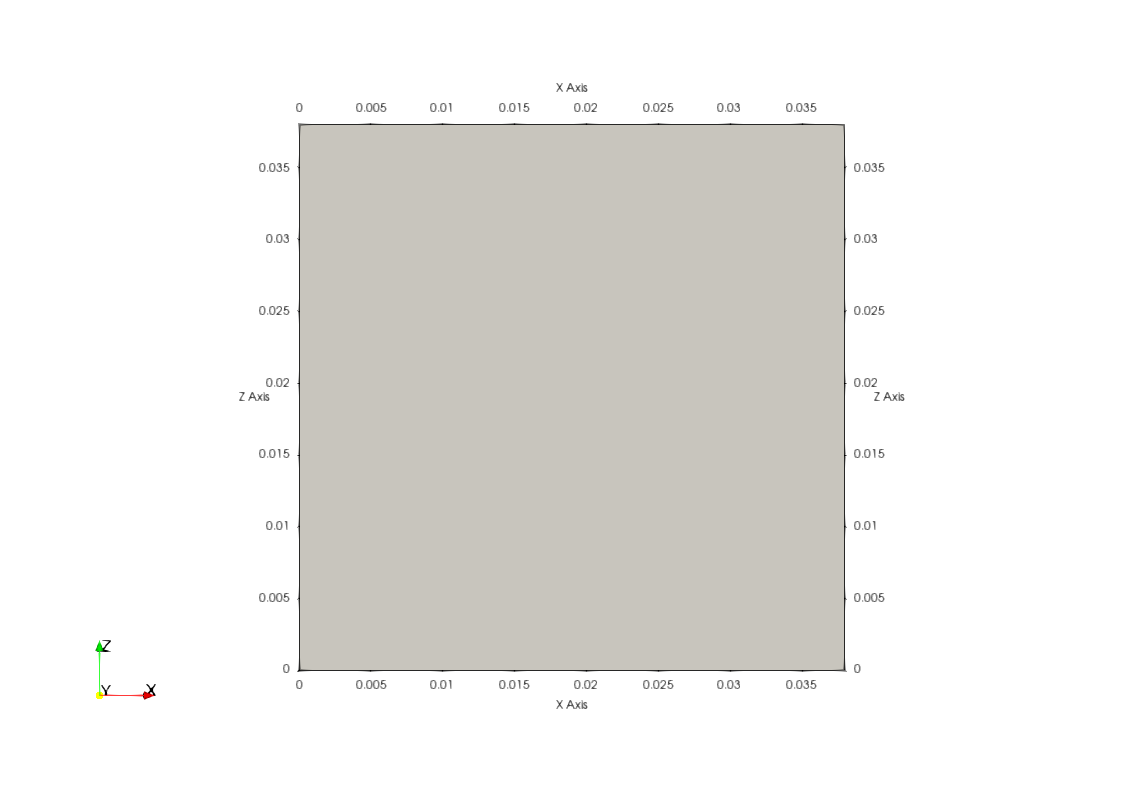
\includegraphics[width=.55\linewidth]{CF_GEOM.png}	
	\label{3.2fig}
	\caption{Geometry of the case.}
\end{figure} 

\subsection{Hypotheses And Assumptions}
To carry out the problem-being, a series of assumptions are taken into account in order to simplify the solving of the fluid equations involved.
\newline
\textbf{Laminar regime:} The Reynolds number, computed from the maximum velocity is not high enough to consider turbulent effects. 
\newline
\textbf{Convective heat transfer:} To determine whether the heat transfer is assumed to be convective, the Prandtl number and the Rayleigh number should be assessed.
\newline
The Prandtl number, as the relation between the viscosity and the thermal conductivity of a fluid or, in other words, the correlation between momentum transport and thermal transport capacity is calculated as:
\begin{equation}
\operatorname{Pr}=\frac{v}{\alpha}=\frac{\eta}{\rho \alpha}=\frac{\eta c_{p}}{\lambda}=\frac{\text { momentum transport }}{\text { heat transport }}
\label{3.3}
\end{equation}
where
Thus, a small Prandtl number are owned by free-flowing flows with high thermal conductivitiy.
\newline
On the other hand, the Rayleigh number is referred to the time scale relation between the diffusive and the convective thermal transports. It is thus used to determine wheter the buoyancy-driven natural convection plays an important role in the heat transfer. The dimensionless number is assessed in this context by this form:
\begin{equation}
\mathrm{Ra}_{x}=\frac{g \cdot \beta}{\nu \cdot \alpha} \cdot\left(T_{s}-T_{\mathrm{inf}}\right) \cdot x^{3}
\label{3.4}
\end{equation}
Being \textit{g}, the gravity, \textit{$\beta$}, the coefficient of thermal expansion, \textit{$\nu$}, the kinematic viscosity, \textit{$\alpha$}, the thermal diffusivity, and \textit{$T_{s}$} and \textit{$T_{\mathrm{inf}}$}, the temperature on the wall surface and the temperature of the fluid far from the wall accordingly.
\newline
In the current case-scenario, a Prandtl close to 7 and a Rayleigh of 2517629 determine a convective heat transfer. The values used to estimate the Rayleigh number calculation are: $\beta = 6.734e-5 K^{-1}$, $\nu = 1.003e-6 m^{2}.s^{-1}$, $\alpha = 1.435e-7 m^{2}.s^{-1}$, $T_{s} = 283 K$, $T_{inf} = 273 K$ and $x = 0.038 m$. The values used for the laminar Prandtl number calculation are: $\mu = 0.001003 Kg.m^{-1}.s^{-1}$, $\lambda = 0.6 W.m^{-1}.K^{-1}$ and $C_{p}=4182 J.Kg.K^{-1}$.
\newline
\textbf{Newtonian fluid:} The viscosity of the fluid is assumed to be constant.
\newline
\textbf{Thermophysical properties:} specific heat, \textit{$C_p$}, the thermal expansion coefficient, \textit{$\beta$}, thermal conductivity, \textit{$\kappa$}, kinematic viscosity, \textit{$\nu$} are assumed to be non-dependent of temperature. However, the density will be dependent of temperature so as it plays an important role in the buoyancy effects through the later explained in this section.

The conservative equations used to describe the motion of the fluid along time and space are described next.
\subsection{Governing Equations}
In this section, the governing equations for the used solver are described first.
\newline
The conservation of mass states that the mass flowing into the volume of control (CV) must be equal to the mass flowing out of such volume. 
\begin{equation}
\frac{\partial v}{\partial y}+\frac{\partial w}{\partial z}=0
\label{3.5}
\end{equation}

\subsubsection{Momentum Equation}
Throughout the CV the momentum of the fluid flow is preserved and here below it is expressed for the y-direction and z-direction.
\begin{equation}
	\begin{aligned}
		\frac{\partial(\rho v)}{\partial t}+\operatorname{div}(\rho \mathbf{u} v)=\operatorname{div}(\mu \operatorname{grad} v)-\frac{\partial P}{\partial y}
	\end{aligned}
	\label{3.6}
\end{equation}
\begin{equation}
	\begin{aligned}
		\frac{\partial(\rho w)}{\partial t}+\operatorname{div}(\rho \mathbf{u} w)=\operatorname{div}(\mu \operatorname{grad} w)-\frac{\partial P}{\partial z}+S_{b}
	\end{aligned}
	\label{3.7}
\end{equation}
where in the case of the \textit{Boussinesq approximation} where the density variation is linear:
\begin{equation}
	S_{b} = g\cdot\rho_{r}[1-\beta(T-T_{r})]
	\label{3.8}
\end{equation}
in the case of the implemented polynomial density which accounts for the inversion point as in \cite{bourdillon_2016}:
\begin{equation}
S_{b} = g\cdot[\rho_{r}-\rho(T)]
\label{3.9}
\end{equation}
where the polynomial expression from $\rho$ is:
\begin{equation}
	\begin{aligned}
		\rho(T) &=999.840281167108+0.0673268037314653 \times T \\
		&-0.00894484552601798 \times T^{2} \\
		&+8.78462866500416 .10^{-5} \times T^{3} 
		-6.62139792627547 .10^{-7} \times T^{4}
	\end{aligned}
	\label{3.9a}
\end{equation}
As it will be pointed out later, the native solver uses the Boussinesq approximation to account for the buoyancy effects. However, this linear assumption is only valid as the density variations meet:
\begin{equation}
\frac{\Delta \rho}{\rho_{r}}<<1
\label{3.10}
\end{equation}
Therefore, to account for the inversion points present during the freezing process, a density variation like the described in \ref{3.9a} is implemented in the solver.

\subsubsection{Temperature Equation}
The temperature equation representing the convection phenomena yields as:
\begin{equation}
	\begin{aligned}
	\frac{\partial T}{\partial t}+ \frac{\partial (u_{j} T)}{\partial x_{j}}=\frac{\partial}{\partial x_{j}}\left(\gamma \frac{\partial T}{\partial x_{j}}\right)
	\end{aligned}
	\label{3.11}
\end{equation}

where the thermal diffusivity, $\gamma$, is defined as:
\begin{equation}
	\gamma=\frac{\lambda}{\rho_{r} c_{p}}
	\label{3.12}
\end{equation}

All these equations are regarded by the solver \textit{buoyantBoussinesqPimpleFoam}.
\subsection{Solver descripton. Control Loop}
The \textit{buoyantBoussinesqPimpleFoam} is a solver used to solve non-steady buoyancy-driven fluids by using the Boussinesq approximation as a coupling between density and temperature fields. It considers the fluid as incompressible and uses the PIMPLE algorithm for the pressure-velocity coupling. The flowchart of the integration procedure for the presented solvers \textit{buoyantBoussinesqPimpleFoam} and \textit{icoReactingMultiphaseinterFoam} is presented below:

\tikzstyle{decision} = [diamond, draw, fill=blue!20,
text width=4.5em, text badly centered, node distance=2.5cm, inner sep=0pt]
\tikzstyle{block} = [rectangle, draw, fill=blue!20,
text width=5em, text centered, rounded corners, minimum height=4em]
\tikzstyle{line} = [draw, very thick, color=black!50, -latex']
\tikzstyle{cloud} = [draw, ellipse,fill=red!20, node distance=2.5cm,
minimum height=2em]
\clearpage
\begin{figure}[h!]
	\centering
	\begin{tikzpicture}[scale=1, node distance = 2cm, auto]
	% Place nodes
	\node [block] (init) {Velocity predictor};
	\node [block, below of=init] (identify) {Temperature Equation};
	\node [block, below of=identify] (evaluate) {Pressure Equation};
	\node [block, below of=evaluate] (update) {Velocity Corrector};
	\node [block, left of=evaluate, node distance=3cm] (update1) {PIMPLE LOOP};
	\node [block, right of=evaluate, node distance=3cm] (update2) {PISO LOOP};
	\node [decision, below of=update] (decide) {Residuals satisfied?};
	\node [block, below of=decide, node distance=2.5cm] (stop) {stop};
	% Draw edges
	\path [line] (init) -- (identify);
	\path [line] (identify) -- (evaluate);
	\path [line] (evaluate) -- (update);
	\path [line] (update) -- (decide);
	\path [line] (decide) -| node [near start, color=black] {no} (update1);
	\path [line] (update1) |- (init);
	\path [line] (update) -| node [near start, color=black] {} (update2);
	\path [line] (update2) -- (evaluate);	
	\path [line] (decide) -- node [, color=black] {yes}(stop);
	
	\end{tikzpicture}
	\label{3.3fig}
	\caption{Flowchart of integration procedure. \textit{buoyantBoussinesqPimpleFoam}}
\end{figure}


\subsection{Code implementations}
As described in the \textit{Governing equations} section, the need for a polynomial density expression and a variation of the momentum source terms devoted to reflect the buoyancy effects is derived.
To do so, a new equation of state is implemented within the OpenFoam framework. Now and, in order to take into account this bouyancy forces, the pressure equation is studied. This is beacause in the context of a pressure-velocity corrector scheme, and in the case of ensuring stability and simplifying the boundary conditions definition, the modified pressure, \textit{$p_{rgh}$}, within the pressure equation implementation, is the term that accounts for the gravity terms.
\newline
Here, it is presented a general form of a momentum equation with the continuity equation corresponding to a incompressible flow.  
\begin{equation}
\left\{\begin{array}{l}
\frac{\partial (\rho \textbf{v})}{\partial t}+\nabla \cdot(\rho \textbf{v} \otimes \textbf{v})=-\nabla p+ \nabla \cdot(\mu (\nabla \textbf{v}+\nabla \textbf{v}^{T})) \\
\nabla \cdot \textbf{v}=0
\end{array}\right.
	\label{3.13}
\end{equation}
From this general equation, it will be given the term $H(\textbf{u})$, as later on will be needed for the pressure equation calculation.
\newline
Therefore, this term comes from considering the linearization of the advective term under the assumption of small Courant numbers (Co < 1). Leading the term $\textbf{v}^{0}\cong\textbf{v}$. 
\begin{equation}
\begin{aligned}
\int_{\Omega} \nabla \cdot\left(\textbf{v} \otimes \textbf{v}^{0}\right) d \Omega & \cong \sum_{f} \textbf{v}_{f} \textbf{v}_{f}^{0} \cdot \textbf{S}_{f} \\
&=\sum_{f} F^{0} \textbf{v}_{f} \\
&=a_{P} \textbf{v}+\sum_{f} a_{N} \textbf{v}_{N}
\end{aligned}
\label{3.14}
\end{equation}

\begin{equation}
a_{P} \textbf{v}_{P}=\textbf{H}(\textbf{v})-\nabla p
\label{3.15}
\end{equation}
\begin{equation}
\textbf{H}(\textbf{v})=\underbrace{-\sum_{f} a_{N} \textbf{v}_{N}}_{\text {Diagonal term }}+\underbrace{\frac{\textbf{v}^{0}}{\Delta t}}_{\text {Off-diagonal term }}
\label{3.16}
\end{equation}
where $\textbf{v}^{0}$ is the velocity at previous time-step and $F^{0}$ is the face flux at the previous time-step.
\newline
In addition, by discretizing the continuity equation, it is possible to get the final form of the pressure equation.
\newline
So as to give stability to the solution and to simplify the boundary conditions definition \cite{berberovic_van hinsberg_jakirlic_roisman_tropea_2009}, a modified pressure is defined as,
\begin{equation}
p_{r g h}=p-\rho_{r} \textbf{g} \cdot \textbf{x} + \rho(T) \textbf{g} \cdot \textbf{x}
\label{3.17}
\end{equation}
being, the pressure gradient the next expression,
\begin{equation}
-\nabla p+\rho_{r} \textbf{g}=-\nabla p_{r g h}-\textbf{g} \cdot \textbf{x} \nabla \rho_{r} + \textbf{g} \cdot \textbf{x} \nabla \rho(T) + \rho(T) \textbf{g}
\label{3.18}
\end{equation}
and rearranging terms, 
\begin{equation}
	-\nabla p+\rho_{r} \textbf{g} + \textbf{g} \cdot \textbf{x} \nabla \rho_{r} - \textbf{g} \cdot \textbf{x} \nabla \rho(T) - \rho(T) \textbf{g}=-\nabla p_{r g h}
	\label{3.19}
\end{equation}
If one tries to describe the discretized pressure equation in \textit{buoyantBoussinesqPimpleFoam}, there is a first term called \textbf{phig}, which is,
\begin{equation}
	\Phi_{f}^{\nu+1}=\Phi_{u}^{\nu+1} - \left[(\textbf{g} \cdot \textbf{x})_{f}\left(\nabla \rho_{r}{ }^{n+1}\right)_{f}+(\textbf{g} \cdot \textbf{x})_{f}\left(\nabla \rho(T){ }^{n+1}\right)_{f}\right]\frac{\left|\textbf{S}_{f}\right|}{\left(a_{P}\right)_{f}}
	\label{3.20}
\end{equation}
A face flux calculated by the term \textbf{H}(\textbf{v}), appearing in equation \ref{3.16}
\begin{equation}
\Phi_{u}^{\nu+1}=\Phi_{f}^{\nu+1} + \left(\frac{H\left(\textbf{v}^{\nu}\right)}{a_{P}}\right)_{f} \cdot \textbf{S}_{f}+\left(\frac{1}{a_{P}}\right)_{f}\operatorname{ddt} \operatorname{PhiCorr}\left(\textbf{v}^{\nu}, \Phi^{\nu}\right)
\label{3.21}
\end{equation}
where $\operatorname{ddt} \operatorname{PhiCorr}$ is a flux adjustment due to the time-step. This is resolved by applying a \textit{Rhie-Chow interpolation}, \cite{rhie_chow_1983}, the next term in the pressure equation, \textbf{phiHbyA}, reads as,
\begin{equation}
\Phi_{f}^{\nu+1}=\Phi_{f}^{\nu+1}-\left[\left(\frac{1}{a_{P}}\right)_{f}\left(\vec{\nabla} p_{r g h}\right)_{f}\right] \cdot \textbf{S}_{f}
\label{3.22}
\end{equation}
The \textbf{$p_{rgh}$} term is thus assembled as,
\begin{equation}
\sum_{f}\left[\left(\frac{1}{a_{P}}\right)_{f}\left(\vec{\nabla} p_{r g h}^{\nu+1}\right)_{f}\right] \cdot \vec{S}_{f}=\sum_{f} \Phi^{\nu+1}
\label{3.23}
\end{equation}
The flux, \textit{$\phi$}, is adjusted by the \textbf{$p_{rgh}$} term yielding the following expression,
\begin{equation}
\Phi_{f}^{\nu+1}=\Phi_{f}^{\nu+1}-\left[\left(\frac{1}{a_{P}}\right)_{f}\left(\vec{\nabla} p_{r g h}\right)_{f}\right] \cdot \textbf{S}_{f}
\label{3.24}
\end{equation}
\begin{equation}
\begin{aligned}
	\Phi_{f}^{\nu+1}=&\Phi_{f}^{\nu+1}+\biggl[\left(\frac{1}{a_{P}}\right)_{f}\biggl[(-\nabla p)_{f}+ (\textbf{g} \cdot \textbf{x})_{f}\left(\nabla \rho_{r}{ }^{n+1}\right)_{f}-(\textbf{g} \cdot \textbf{x})_{f}\left(\nabla \rho(T){ }^{n+1}\right)_{f}\\
	&+ (\rho_{r}{ }^{n+1} \textbf{g})_{f}-(\rho(T){ }^{n+1} \textbf{g})_{f} \biggr]\biggr] \cdot \textbf{S}_{f}
\end{aligned}
\label{3.25}
\end{equation}
Finally, the velocity calculated at the center of the volume reads as,
\begin{equation}
\textbf{v}^{\nu+1}=\textbf{v}^{\nu+1} +\frac{1}{a_{P}}\mathcal{R}\left[\left(\Phi^{\nu+1} f-\Phi_{u}^{\nu+1} f\right)\left(a_{P}\right)_{f}\right]
\label{3.26}
\end{equation}
where $\mathcal{R}$ is an operator used to recover cell-centered fields from fields given as fluxes at faces.
Then, the static pressure, \textit{p}, is reconstructed from \textit{$p_{rgh}$}, leading the expression,

\begin{equation}
p = p_{r g h} + (\rho_{r}-\rho(T))\textbf{g}\cdot \textbf{x}
\label{3.27}
\end{equation}
 
\subsection{Case Setup}
Once the implementation is done, a first case is studied with the existing solver, \textit{buoyantBoussinesqPimpleFoam}. 
The boundary conditions, thermophysical properties and some other solver parameters are described along the following subsections.
\newline
As commented before, all studies are calculated on a computational domain of \textit{38mm x 38mm}. 
\begin{figure}[h]
	\label{3.43}	\centering	
	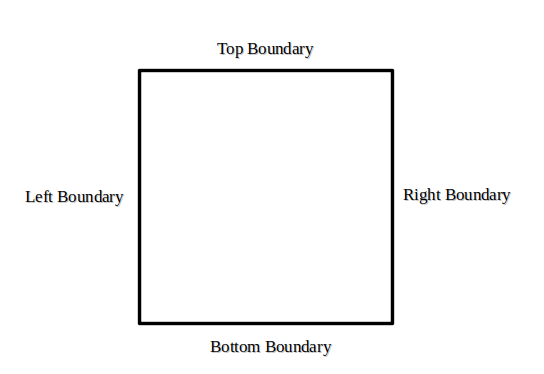
\includegraphics[width=0.6\textwidth]{domain.png}
	\caption{Setting of computational domain.}
\end{figure} 

\subsubsection*{Boundary conditions}
Five boundaries are defined in the current case:
\newline
\textbf{Left:} is considered a wall with a fixed value of temperature. This is the hot wall. No velocity is prescribed.
\newline
\textbf{Right:} considered to be the cold wall with a fixed temperature. No velocity is prescribed.
\newline
\textbf{Top:} this is considered the top wall and it is adiabatic, thus, no heat transfer is assumed and zero gradient is applied. No velocity is applied.
\newline 
\textbf{Bottom:} This shares similar conditions as the top wall.
\newline
\textbf{frontAndBack:} this uses a symmetry plane condition in the z direction since the problem is considered to be 2-dimensional. For such boundary type, no more conditions need to be prescribed.
\begin{table}[h!]
	\begin{tabular}{@{}lllll@{}}
		\toprule[1pt]
		\textbf{Boundary} & \textbf{Conditions}  \\ \midrule[2pt]
		Left & $T_{l}=283, v_{l} = 0   $  \\
		Right & $T_{r}=273, v_{r} = 0 $ \\
		Top & $\frac{\partial T_{u}}{\partial n} = 0, v_{u} = 0$  \\
		Bottom & $\frac{\partial T_{b}}{\partial n} = 0, v_{b} = 0$  \\ \bottomrule[1pt]		
	\end{tabular}
	\centering
	\caption{Boundary conditions for natural convection case.}	
	\label{fig:boundaryCdsNaturalConvection}
\end{table}


\subsubsection*{Thermophysical properties}
\begin{table}[h!]
	\begin{tabular}{@{}lllll@{}}
		\toprule[1pt]
		\textbf{Water properties} & \textbf{Symbol} & \textbf{Values} & \textbf{Units} &  \\ \midrule[2pt]
		Density & $\rho_r$ & 999.8 & $kg.m^{-3}$ \\
		Dynamic viscosity & $\mu$ & 0.001003 & $kg.m^{-1}.s^{-1}$ \\
		Thermal conductivity & $\lambda$ & 0.6 & $W.m^{-1}.K^{-1}$ \\
		Heat capacity & $C_p$ & 4182 & $J.kg.K^{-1}$ \\		 
		Gravitational acceleration & $g$ &  9.81  & $m.s^{-2}$ \\
		Thermal diffusivity & $\gamma$ &  1.435e-7  & $m^{2}.s^{-1}$ \\		
		Thermal expansion coefficient & $\beta$ &  6.734e-5  & $K^{-1}$ \\	
		Laminar Prandtl number & $P_r$ &  6.99  & - \\
		Reference temperature & $T_r$ &  6.734e-5  & $K$ \\ \bottomrule[1pt]		
	\end{tabular}
	\centering
	\caption{Water properties for natural convection.}	
	\label{fig:waterProperties}
\end{table}

\subsubsection*{Solver parameters}
\begin{table}[h!]
	\begin{tabular}{@{}lllll@{}}
		\toprule[1pt]
		\textbf{Modeling Term} & \textbf{Keyword} & \textbf{Scheme} & \textbf{Remarks} &  \\ \midrule[2pt]
		Time derivatives & ddtSchemes    & Euler   &  \\
		Divergence term   &    &    &  \\
		Gradient term    & gradSchemes    &  Gauss linear  &  \\
		Laplacian term   &  laplacianSchemes    &  Gauss linear uncorrected   &  \\		 
		Others   		 & snGradSchemes    & uncorrected  &  \\ 
		&    			   interpolationSchemes    & linear  &  \\ \bottomrule[1pt]		
	\end{tabular}
		\centering
		\caption{Discretization schemes.}	
		\label{fig:boat3}
\end{table}
\clearpage
\begin{table}[h!]
	\begin{tabular}{@{}lllll@{}}
		\toprule[1pt]
		\textbf{Equation} & \textbf{Linear Solver} & \textbf{Smoother/Preconditioner} & \textbf{Tolerance} &  \\ \midrule[2pt]
		Pressure correction equation & PCG & DIC & 1e-8 \\
		Momentum equation & PBiCGStab & DILU  & 1e-6 \\
		Temperature equation & PBiCGStab & DILU  & 1e-6 \\\bottomrule[1pt]		
	\end{tabular}
	\centering
	\caption{Solvers for the discretised equations.}	
	\label{fig:boat4}
\end{table}
\begin{table}[h!]
	\begin{tabular}{@{}lllll@{}}
		\toprule[1pt]
		\textbf{Parameter} & \textbf{Value} & \textbf{Remarks} & \\ \midrule[2pt]
%		nAlphaCorr & PCG & DIC &  \\
%		nAlphaSubCycles & smoothSolver & symGaussSeidel  &  \\
%		cAlpha & smoothSolver & symGaussSeidel  &  \\
		momentumPredictor &  no    &    &  \\		 
		nOuterCorrectors &  1   &    &  \\ 
		nNonOrthogonalCorrectors &  0   &    &  \\ 		
		nCorrectors & 2	&    &  \\ \bottomrule[1pt]		
	\end{tabular}
	\centering
	\caption{Parameters for the discretised equations.}	
	\label{fig:boat5}
\end{table}

\subsection{Validation of Results and Conclusions}
\begin{figure}[h!]
	\centering
	\begin{subfigure}{\linewidth}
	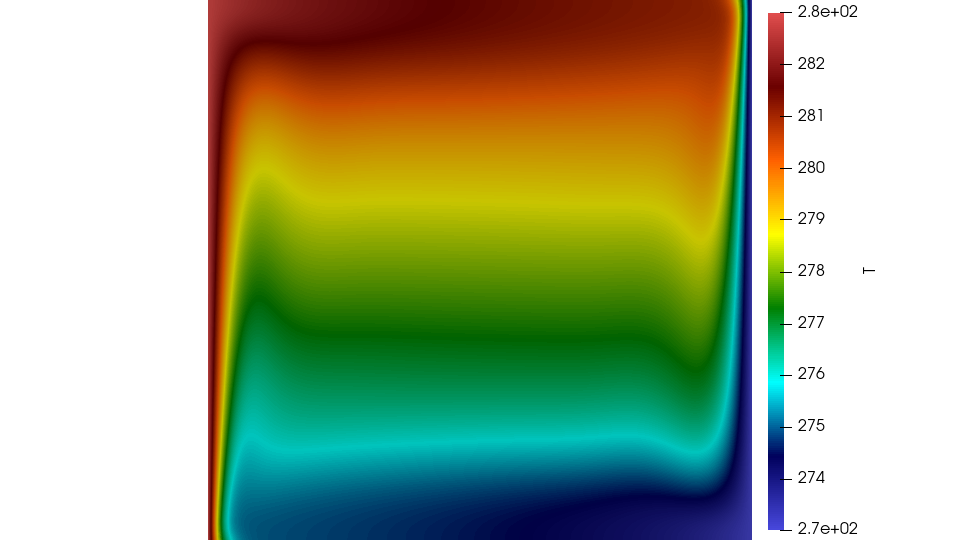
\includegraphics[width=.55\linewidth]{BBPF_T_1500s.png}\hfill
	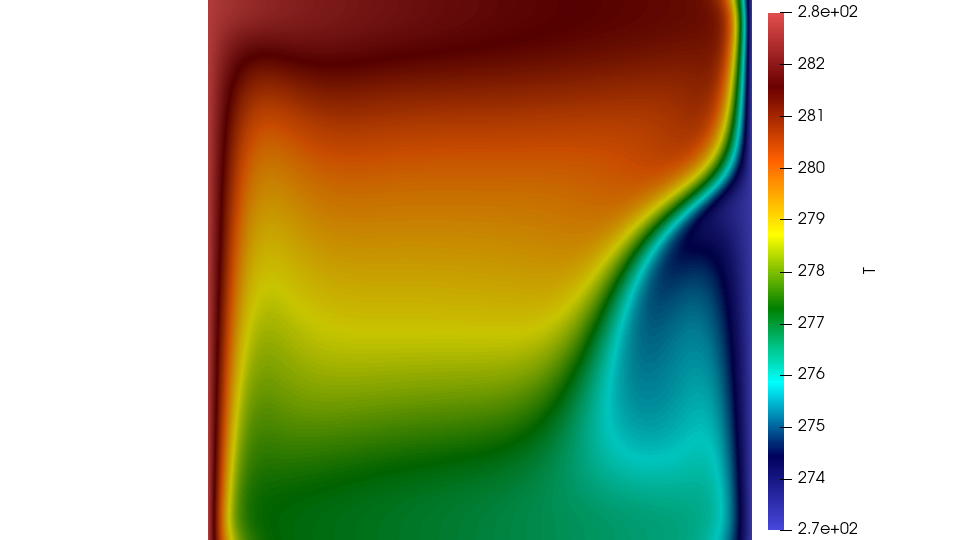
\includegraphics[width=.55\linewidth]{CF_T_1500s_comp.png}	
	\caption{Temperature magnitude comparison at t = 1500s. Left: BuoyantBoussinesqPimpleFoam. Right: NCMF}
	\label{BBPF_NCMF}
	\end{subfigure}\par\medskip
	\begin{subfigure}{\linewidth}
	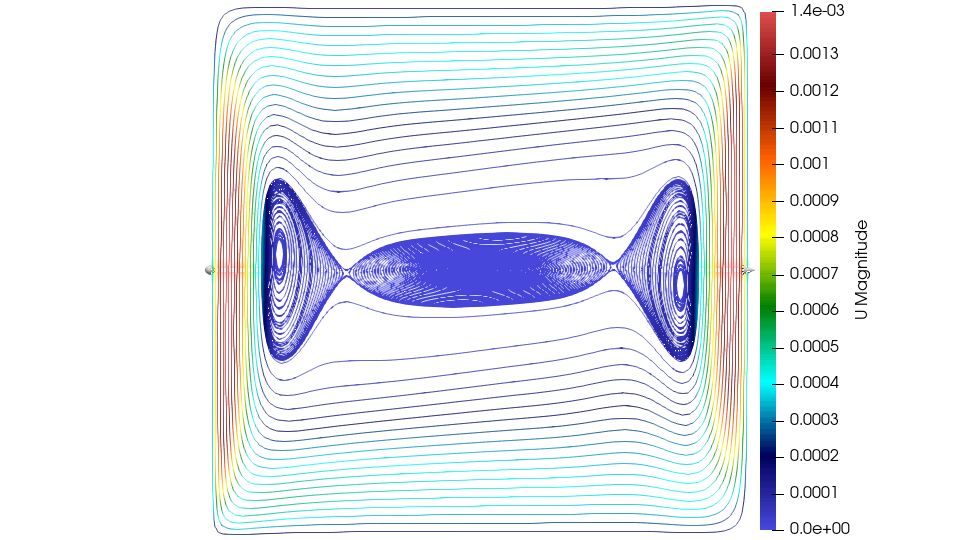
\includegraphics[width=.55\linewidth]{BBPF_U_1500s.png}\hfill
	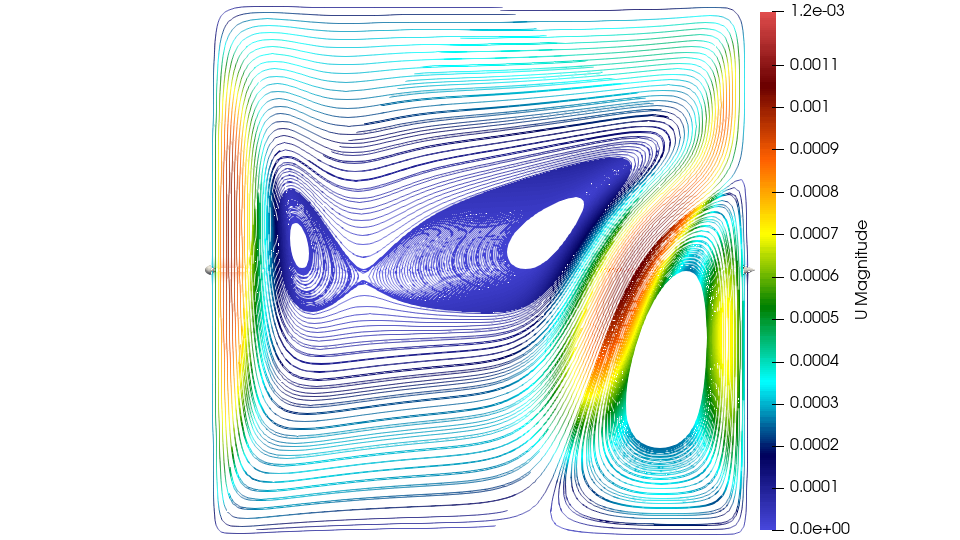
\includegraphics[width=.55\linewidth]{CF_U_1500s_comp.png}	
	\caption{Velocity magnitude comparison at t = 1500s. Left: BuoyantBoussinesqPimpleFoam. Right: NCMF}
	\end{subfigure}\par\medskip
	\caption{Comparison between BuoyantBoussinesqPimpleFoam and NCMF*}
\end{figure} 
NCMF*: Natural convection modified solver.
\newline
In order to compare consistently the obtained results with those of the literature, the following dimensionless values are pointed out:
\begin{equation}
\tilde{T}=\frac{T-T_{\text {cold }}}{T_{\text {hot }}-T_{\text {cold }}}=\frac{T-273}{10}
\label{3.28}
\end{equation}
\begin{equation}
\tilde{x}=\frac{x}{\ell}=\frac{x}{38 \times 10^{-3}}
\label{3.29}
\end{equation}
\begin{equation}
\tilde{v}=\frac{v \ell}{\gamma}=\frac{v 38 \times 10^{-3}}{1.435 \times 10^{-7}}
\label{3.30}
\end{equation}
\begin{equation}
\tilde{u}=\frac{u \ell}{\gamma}=\frac{u 38 \times 10^{-3}}{1.435 \times 10^{-7}}
\label{3.31}
\end{equation}
\begin{equation}
\tilde{t}=\frac{t \gamma}{\ell^{2}}=\frac{t \times 1.435 \times 10^{-7}}{1.444 \times 10^{-6}}
\label{3.32}
\end{equation}
\begin{equation}
\tilde{y}=\frac{y}{\ell}=\frac{y}{38 \times 10^{-3}}
\label{3.33}
\end{equation}
\clearpage
\begin{figure}[h!]
	\begin{subfigure}{0.50\textwidth}
		\centering
		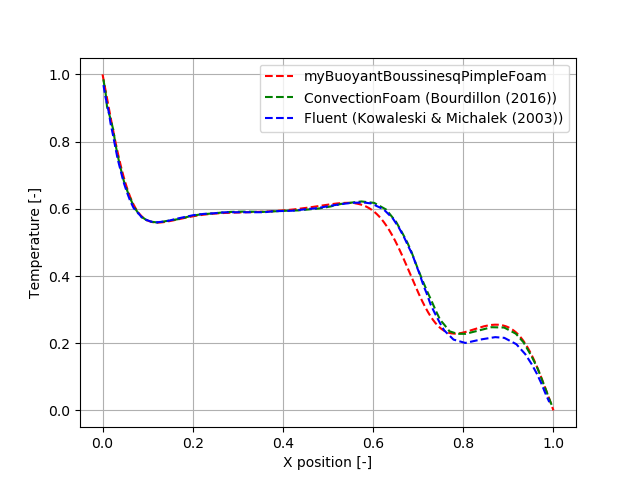
\includegraphics[width=\linewidth]{temperature_xpos_conv.png}\hfill
		\caption{Temperature along horizontal line.} \label{3.4afig}
	\end{subfigure}
	\hfill
	\begin{subfigure}{0.50\textwidth}
		\centering
		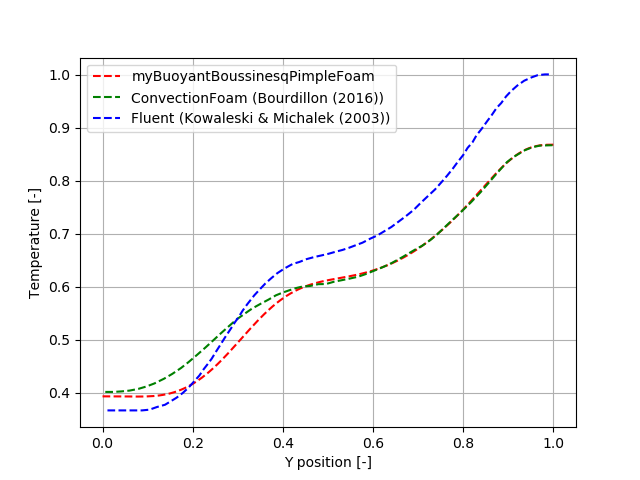
\includegraphics[width=\linewidth]{temperature_ypos_conv.png}	
		\caption{Temperature along vertical line.}\label{3.4bfig}
	\end{subfigure}
	\begin{subfigure}{0.50\textwidth}
		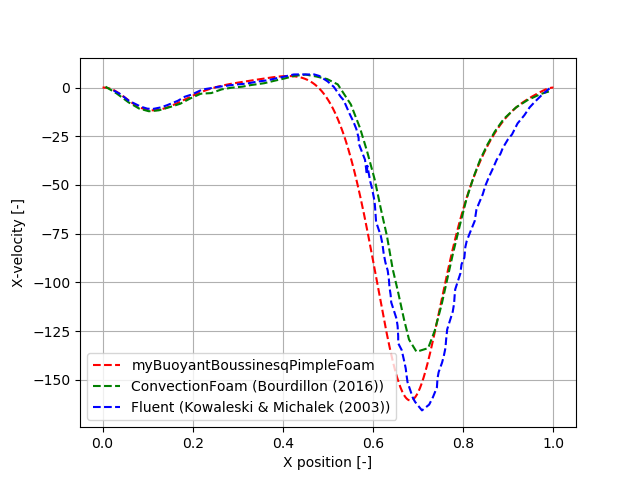
\includegraphics[width=\linewidth]{xvel_xpos_conv.png}\hfill
		\caption{U-velocity along horizontal line.}\label{3.4cfig}
	\end{subfigure}
	\begin{subfigure}{0.50\textwidth}
	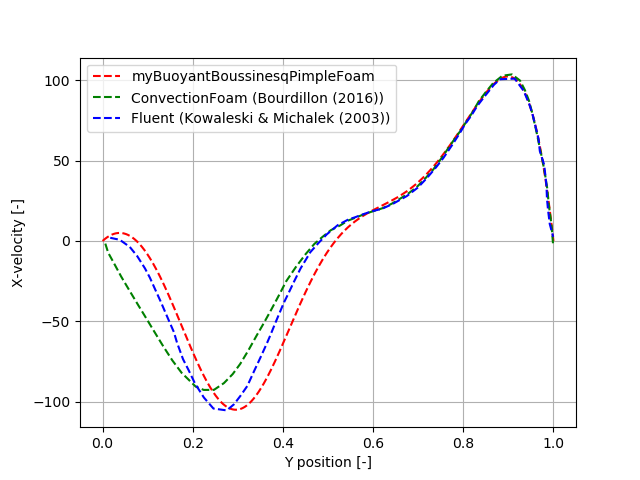
\includegraphics[width=\linewidth]{xvel_ypos_conv.png}	
	\caption{U-velocity along vertical line.}\label{3.4dfig}
	\end{subfigure}
	\begin{subfigure}{0.50\textwidth}
	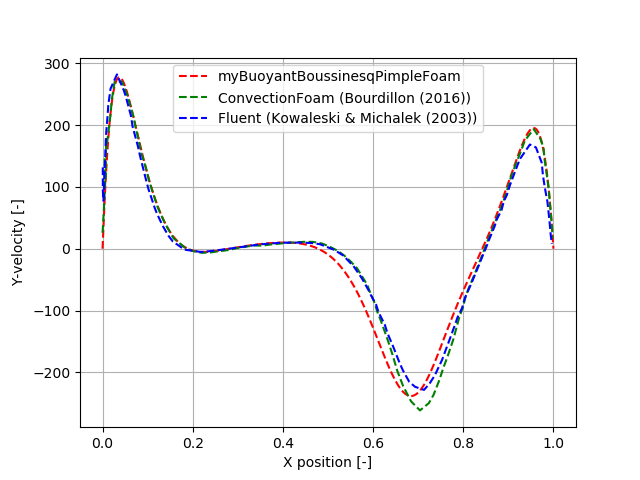
\includegraphics[width=\linewidth]{yvel_xpos_conv.png}\hfill	
	\caption{V-velocity along horizontal line.}\label{3.4efig}
	\end{subfigure}
	\begin{subfigure}{0.50\textwidth}
	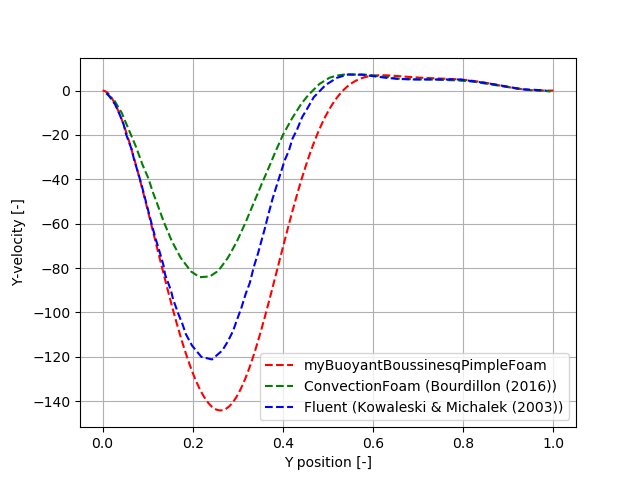
\includegraphics[width=\linewidth]{yvel_ypos_conv.png}	
	\caption{V-velocity along vertical line.}\label{3.4ffig}
	\end{subfigure}
	\caption{Adimensional magnitudes comparison.}
	\label{3.4fig}
\end{figure} 
\begin{table}[h!]
	\begin{tabular}{@{}lllll@{}}
		\toprule[1pt]
		\multicolumn{1}{c}{\textbf{t = 100s}} & \multicolumn{1}{c}{\textbf{t = 250s}} & \multicolumn{1}{c}{\textbf{t = 1500s}} \\ \midrule[2pt] 
		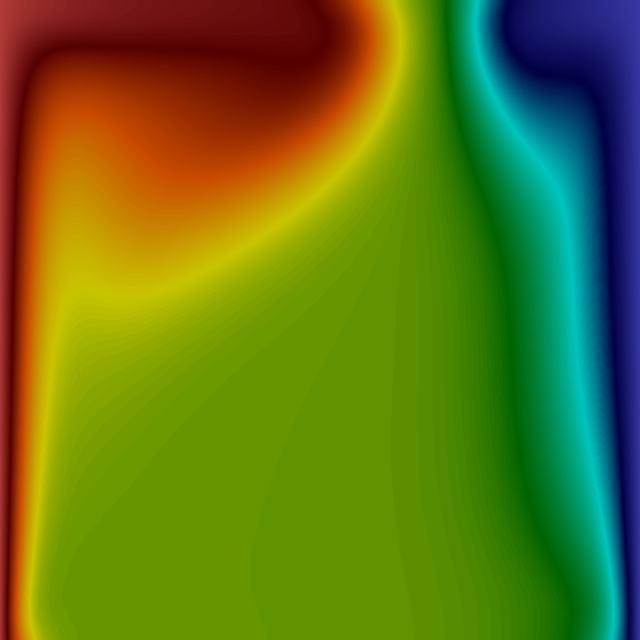
\includegraphics[width=.25\linewidth]{CF_T_100s.png} & 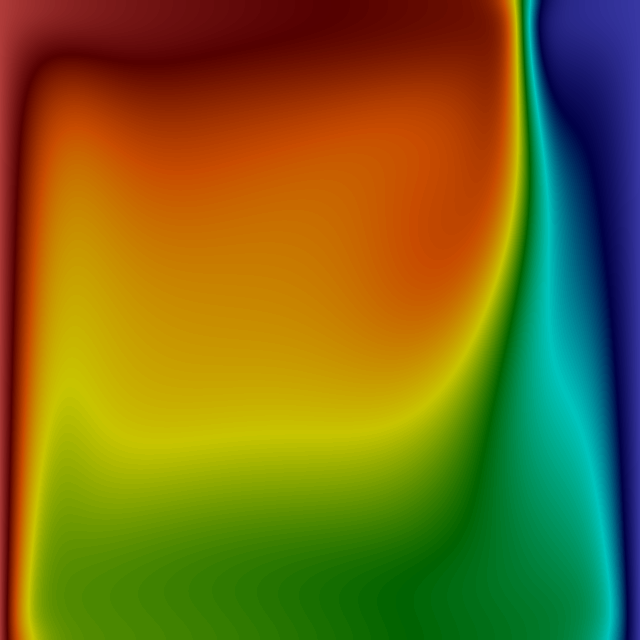
\includegraphics[width=.25\linewidth]{CF_T_250s.png} & 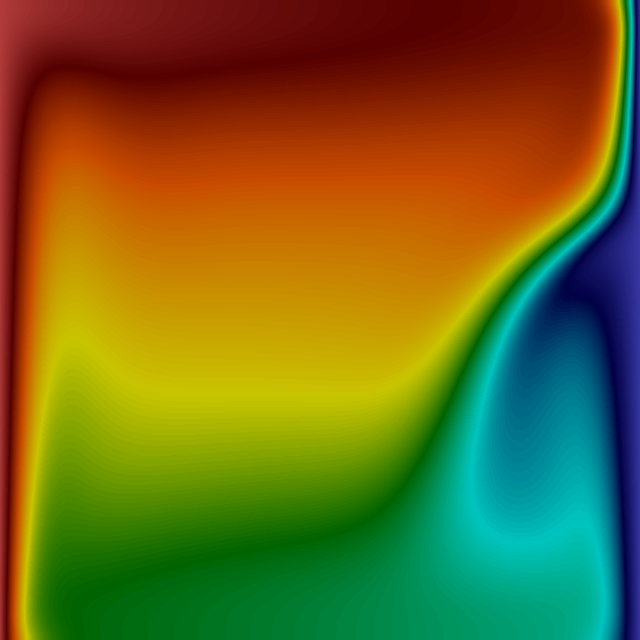
\includegraphics[width=.25\linewidth]{CF_T_1500s.png} & 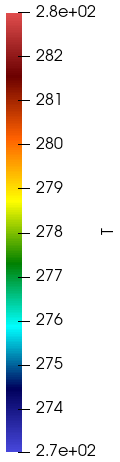
\includegraphics[width=.0658\linewidth]{t.png} \\
		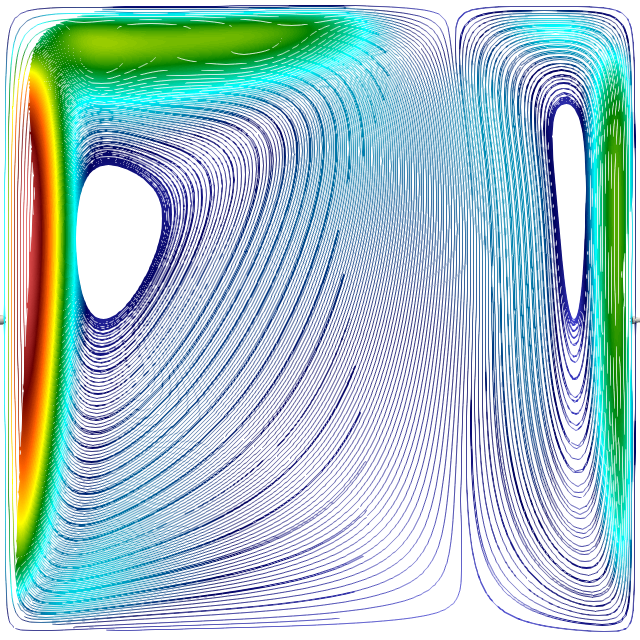
\includegraphics[width=.25\linewidth]{CF_U_100s.png} & 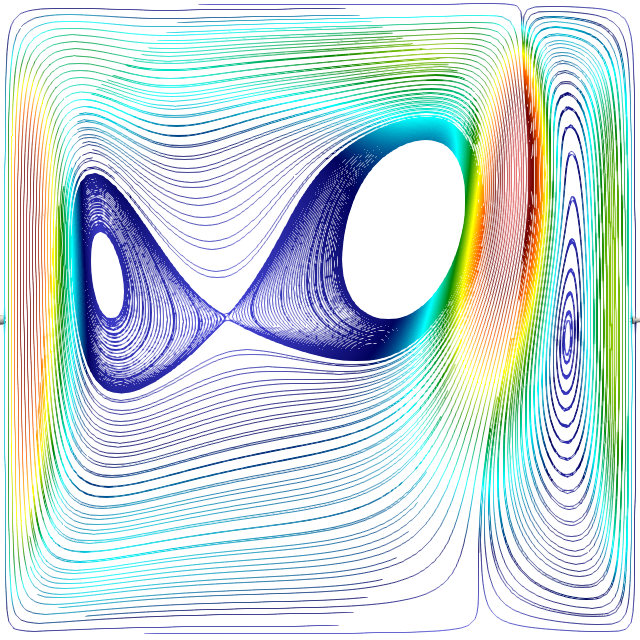
\includegraphics[width=.25\linewidth]{CF_U_250s.png} & 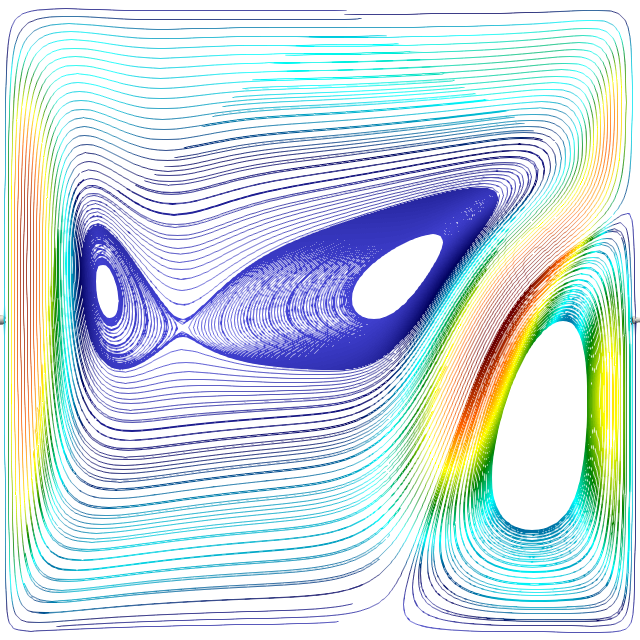
\includegraphics[width=.25\linewidth]{CF_U_1500s.png} & 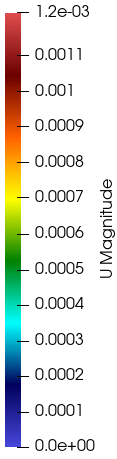
\includegraphics[width=.0658\linewidth]{u.png} \\
		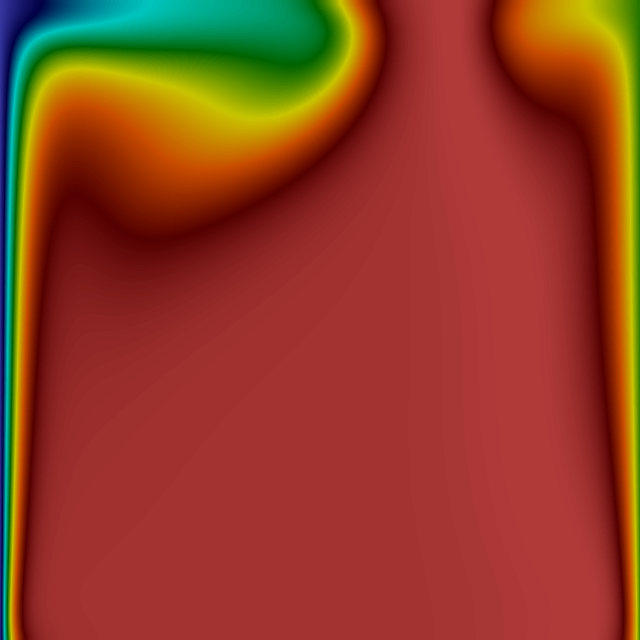
\includegraphics[width=.25\linewidth]{CF_rho_100s.png} & 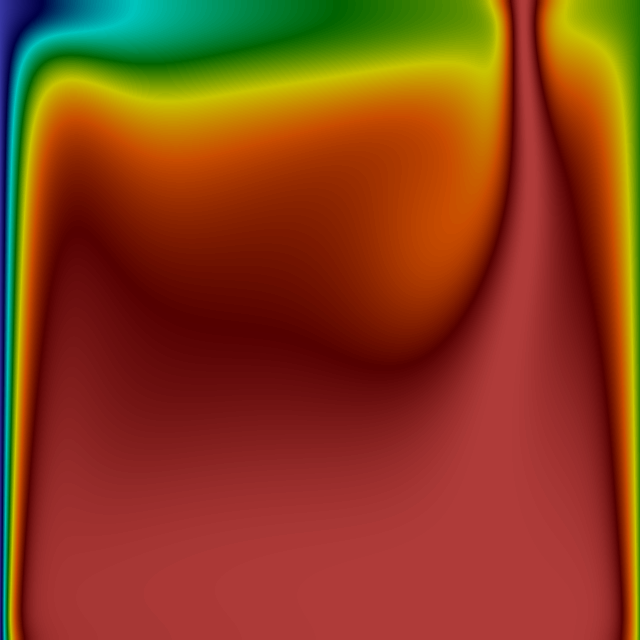
\includegraphics[width=.25\linewidth]{CF_rho_250s.png} & 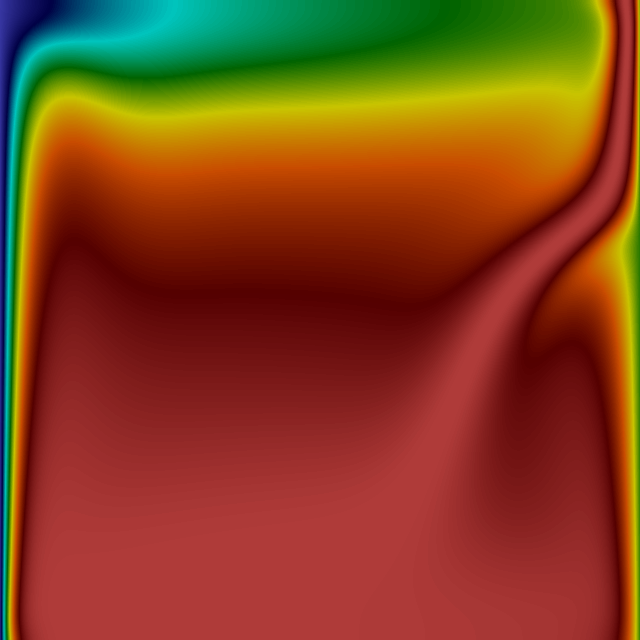
\includegraphics[width=.25\linewidth]{CF_rho_1500s.png} & 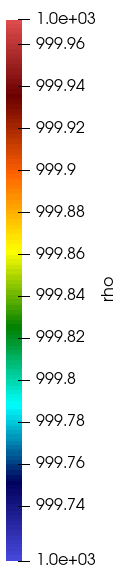
\includegraphics[width=.0558\linewidth]{rho.png} \\ \bottomrule[1pt]		
	\end{tabular}
	\centering
	\caption{Numerical results of Natural convection modified solver between \textit{t = 100s} and \textit{1500s}.}	
	\label{fig:resultsNCMF}
\end{table}

\clearpage
\section{OpenFOAM: IcoReactingMultiphaseInterFOAM. Phase-Change Process}
The solidification process is assessed in this section with two elaborated models. Both of the models are implemented within a multiphase solver based on the volume of fluid technique. This technique aims to capture interface and enhances contact angle and surface tension for each phase. Thus, the first model is based on the coupling of the VOF and the enthalpy-porosity method. To accomplish the inclusion of the enthalpy-porosity method, a library in which the latent heat is implemented as an explicit source term for the energy equation in the solver. On the other hand, the second model uses the VOF method combined with a semi-empirical model based on the work of Lee. The empirical constant is adapted here to be used in conjunction with the use of the \textit{Classical Nucleation Theory}.
\section{Case Description.}
Two regular geomtries are created: a squared cavity, used in the pure convection case and cylindrical plane geometry. Both geometries test both solidification models.
\begin{figure}[h!]
	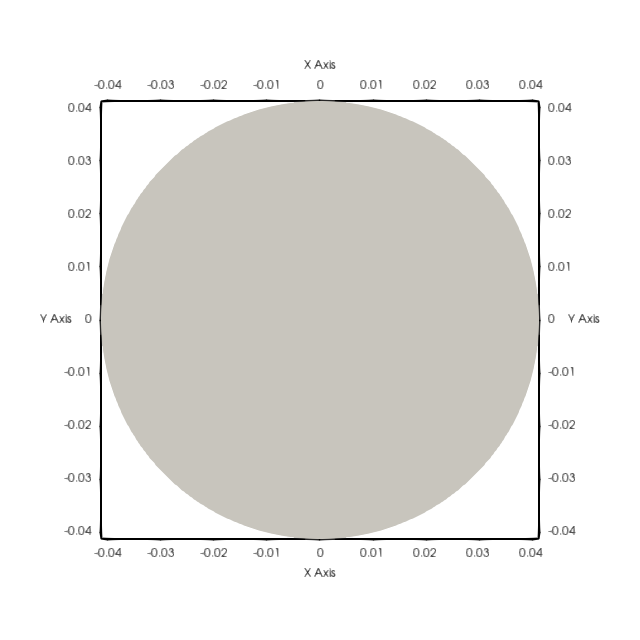
\includegraphics[width=0.6\linewidth]{cylinder_geom.png}\hfill	
	\caption{Cylinder.}\label{3.4efig}
\end{figure}

\subsection{Hypotheses And Assumptions}
To carry out the phase-transition process, some assumptions are taken into account so as to simplify the multiphysics ocurring during such arising phenomena. 
\subsubsection*{Two phase properties}
Within a multiphase framework, a model reflects a jump in properties through the interphase. Thus, a smooth transition between phase properties must be achieved.
\begin{equation}
\lambda=\lambda_{\ell} \alpha_{\ell}+\lambda_{s} f_{s}
\label{3.34}
\end{equation}
\begin{equation}
C_{p}=C_{p_{\ell}} \alpha_{\ell}+C_{p_{s}} f_{s}
\label{3.35}
\end{equation}
\begin{equation}
\mu=\mu_{\ell} \alpha_{\ell}+\mu_{s} f_{s}
\label{3.36}
\end{equation}

In the case of polynomial density variation it is settled in a similar manner. The polynomial is not thought to suit negative temperatures, and when the problem is within this range, the density should take ice's density.
\begin{equation}
\rho(T)^{\prime}=\rho(T) \alpha_{\ell}+\rho_{s} f_{s}
\label{3.37}
\end{equation}

\subsection{Governing Equations}
The solution of the system of equations given by the multiphase solver relies on a pressure-velocity coupling loop based on PISO (\textit{Pressure-Implicit with Splitting of Operators}). In order to give more stability to the solution and to simplify the boundary conditions, the pressure is treated by using a modified pressure:
\newline
Therefore, due to the commented before, the buoyancy terms appearing on the RHS of the momentum equation, are implemented on the pressure equation.

\subsubsection{Momentum Equation}
The momentum equation has the same terms as per each one of the models.
\subsubsection{Energy Equation}
On the other side, the energy equation slightly differs from one model to the other. As pointed out before, here there are recalled both energy equations.

\subsection{Solver description. Control Loop}
IcoReactingMultiphaseInterFoam solver is a multiphase, multicomponent incompressible solver based on volume of fluid method. The solver captures the interfaces and includes contact angle and surface tension effects for each phase. Moreover, this solver supports mass and heat transfer across phases.
\subsection{Phase models}
The solver allows for the use of three phase model types:
\begin{itemize}
	\item \textbf{pureStaticSolidPhaseModel:} For pure static phase, like a solid.
	\item \textbf{pureMovingPhaseModel:} For pure moving phase, like a fluid.
	\item \textbf{multiComponentMovingPhaseModel:} For multi-component moving phase, like a multi-component fluid.
\end{itemize}
In the current case-scenario, the \textit{pureStaticSolidPhaseModel} is selected for the solid phase and the \textit{pureMovingPhaseModel} is used for the liquid phase. 
\subsection{Mass transfer models}
For each pair of phases, two mass transfer models might be used:
\begin{itemize}
	\item \textbf{Lee model:} Used for solid melting and liquid solidification.
	\item \textbf{KineticGasEvaporation:} Used for condensation and evaporation.
\end{itemize}
In this thesis, only the Lee model will be considered for further explanation.








\subsection{Code implementations}
Within the entrophy-porosity model, the source term belonging to the calculation of the latent heat is added within the OpenFOAM framework. The energy equation of the solver shown in [ref].
\begin{figure}[h!]
	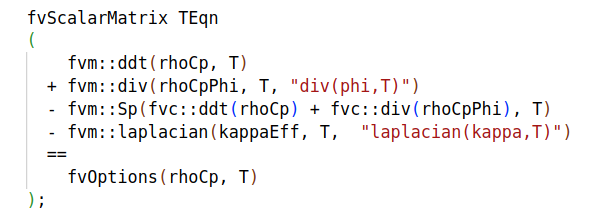
\includegraphics[width=0.6\linewidth]{TEqn.png}\hfill	
	\caption{Energy equation of IcoReactingMultiphaseInterFoam.}\label{}
\end{figure}
In the RHS of the equation, the solver calls the library \textit{mySolidificationMeltingSource} that calculates the latent heat source term as it appears in the Energy equation shown below.
\begin{figure}[h!]
	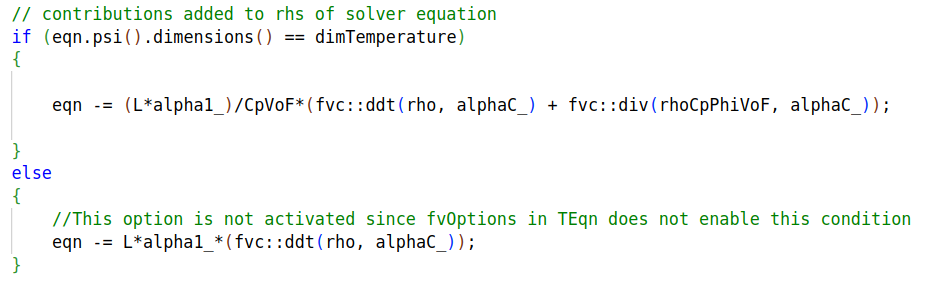
\includegraphics[width=0.6\linewidth]{solidificationMeltingSource.png}\hfill	
	\caption{Latent heat source term present in mySolidificationMeltingSource library.}\label{}
\end{figure}
This library is adapted to be used in this solver. It exists in the context of being used for other solvers. Here, the alpha variable showing up in the calculation is obtained through a linear expression that gives the amount of energy contained in the fluid cell above the melting point. This is divided by the latent heat to obtain the liquid fraction. Then, this fraction is constained between 0 and 1. 
\newline
The latent heat source term is afterwards weighted by the volume fraction calculated by means of the transport equation in the context of the volume of fluid method as it appears in Richter et al. 
\newline

The \textbf{rhoCpPhi} term, which is called in this library, is created in \textit{createFields.H} as a variable field so that it can be called from everywhere within the code.
 
The implemented library can be found in the Appendix \ref{AppendixA}. 

\subsection{Case Setup}
\subsubsection*{Boundary conditions}

For the squared cavity:
The initial conditions for the velocity and temperature fields are inherited from the last timestep of the natural convection case.
\begin{table}[h!]
	\begin{tabular}{@{}lllll@{}}
		\toprule[1pt]
		\textbf{Boundary} & \textbf{Conditions}  \\ \midrule[2pt]
		Left & $\frac{\partial \alpha_{l}}{\partial n} = 0, \frac{\partial \alpha_{s}}{\partial n} = 0    $  \\
		Right & $\alpha_{l} = 1, \alpha_{l} = 0 $ \\
		Upper & $\frac{\partial \alpha_{l}}{\partial n} = 0, \frac{\partial \alpha_{s}}{\partial n} = 0$  \\
		Bottom & $\frac{\partial \alpha_{l}}{\partial n} = 0, \frac{\partial \alpha_{s}}{\partial n} = 0 $  \\ \bottomrule[1pt]		
	\end{tabular}
	\centering
	\caption{Boundary conditions for natural convection case.}	
	\label{fig:boundaryCdsCavity}
\end{table}

For the cylinder:
\begin{table}[h!]
	\begin{tabular}{@{}lllll@{}}
		\toprule[1pt]
		\textbf{Boundary} & \textbf{Conditions}  \\ \midrule[2pt]
		Left & $T_{l}=283, v_{l} = 0   $  \\
		Right & $T_{r}=273, v_{r} = 0 $ \\
		Upper & $\frac{\partial T_{u}}{\partial n} = 0, v_{u} = 0$  \\
		Bottom & $\frac{\partial T_{b}}{\partial n} = 0, v_{b} = 0$  \\ \bottomrule[1pt]		
	\end{tabular}
	\centering
	\caption{Boundary conditions for natural convection case.}	
	\label{fig:boundaryCdsCylinder}
\end{table}
\subsubsection*{Thermophysical properties}
\begin{table}[h!]
	\begin{tabular}{@{}lllll@{}}
		\toprule[1pt]
		\textbf{Water properties} & \textbf{Symbol} & \textbf{Values} & \textbf{Units} &  \\ \midrule[2pt]
		Water density & $\rho_l$ & 999.8 & $kg.m^{-3}$ \\
		Ice density & $\rho_s$ & 916.8 & $kg.m^{-3}$ \\		
		Water kinematic viscosity & $\nu_{l}$ & 1.79e-6 & $m^{2}.s^{-1}$ \\
		Ice kinematic viscosity & $\nu_{s}$ & 2.0e-6 & $m^{2}.s^{-1}$ \\		
		Water thermal conductivity & $\lambda_{l}$ & 0.56 & $W.m^{-1}.K^{-1}$ \\
		Ice thermal conductivity & $\lambda_{s}$ & 2.26 & $W.m^{-1}.K^{-1}$ \\		
		Heat capacity & $C_{p_{l}}=C_{p_{s}}$ & 4202 & $J.kg.K^{-1}$ \\		 
		Gravitational acceleration & $g$ &  9.81  & $m.s^{-2}$ \\
		Thermal diffusivity & $\gamma$ &  1.435e-7  & $m^{2}.s^{-1}$ \\		
		Thermal expansion coefficient & $\beta$ &  6.734e-5  & $K^{-1}$ \\
		Latent heat & $L$ &  335000  & $J.K^{-1}$ \\			
		Laminar Prandtl number & $P_r$ &  6.99  & - \\
		Reference temperature & $T_r$ &  6.734e-5  & $K$ \\
		Darcy's constant & $D_c$ &  10e8  & - \\		 \bottomrule[1pt]		
	\end{tabular}
	\centering
	\caption{Water properties for natural convection.}	
	\label{fig:waterProperties}
\end{table}

\begin{table}[h!]
	\begin{tabular}{@{}lllll@{}}
		\toprule[1pt]
		\textbf{Water nucleation properties} & \textbf{Symbol} & \textbf{Values} & \textbf{Units} &  \\ \midrule[2pt]
		Planck constant & $h$ & 6.63e-34 & $J.s$ \\
		Boltzmann constant & $k_{B}$ & 1.38e-23 & $J.K^{-1}$ \\		
		Gibbs free energy & $\Delta_{gv}$ & 4e-20 & $J$ \\
		Interfacial tension & $\gamma_{yw}$ & 2.91e-2 & $J.m^{-2}$ \\		
		Latent heat per volume & $H_{lv}$ & 3.10e8 & $J.m^{-3}$ \\
		Shape coefficient of nucleation & $\alpha_{ey}$ & 0.0001 & - \\		
		Water molecule per volume & $n_{L}$ &  5.5e4  & $m^{3}$ \\		 \bottomrule[1pt]		
	\end{tabular}
	\centering
	\caption{Water properties for solidification.}	
	\label{fig:waterProperties}
\end{table}


\subsubsection*{Solver parameters}
\begin{table}[h!]
	\begin{tabular}{@{}lllll@{}}
		\toprule[1pt]
		\textbf{Modeling Term} & \textbf{Keyword} & \textbf{Scheme} & \textbf{Remarks} &  \\ \midrule[2pt]
		Time derivatives & ddtSchemes    &    &  \\
		Divergence term    &    &    &  \\
		Gradient term    & gradSchemes    &    &  \\
		Laplacian term   &  laplacianSchemes    &    &  \\		 
		Others   		 & snGradSchemes    &    &  \\ 
		&    			   interpolationSchemes    &    &  \\ \bottomrule[1pt]		
	\end{tabular}
	\centering
	\caption{Discretization schemes.}	
	\label{fig:boat3}
\end{table}
\begin{table}[h!]
	\begin{tabular}{@{}lllll@{}}
		\toprule[1pt]
		\textbf{Equation} & \textbf{Linear Solver} & \textbf{Smoother/Preconditioner} & \textbf{Tolerance} &  \\ \midrule[2pt]
		Pressure correction equation & PCG & DIC &  \\
		Momentum equation & smoothSolver & symGaussSeidel  &  \\
		Volume fraction equation & smoothSolver & symGaussSeidel  &  \\
		&      &    &  \\		 
		&     &    &  \\ 
		&    			       &    &  \\ \bottomrule[1pt]		
	\end{tabular}
	\centering
	\caption{Solvers for the discretised equations.}	
	\label{fig:boat4}
\end{table}
\begin{table}[h!]
	\begin{tabular}{@{}lllll@{}}
		\toprule[1pt]
		\textbf{Parameter} & \textbf{Value} & \textbf{Remarks} & \\ \midrule[2pt]
		nAlphaCorr & PCG & DIC &  \\
		nAlphaSubCycles & smoothSolver & symGaussSeidel  &  \\
		cAlpha & smoothSolver & symGaussSeidel  &  \\
		momentumPredictor &      &    &  \\		 
		nOuterCorrectors &     &    &  \\ 
		nNonOrthogonalCorrectors &     &    &  \\ 		
		nCorrectors &    			       &    &  \\ \bottomrule[1pt]		
	\end{tabular}
	\centering
	\caption{Parameters for the discretised equations.}	
	\label{fig:boat5}
\end{table}

\subsection{Validation of Results and Conclusions}
The validation of the phase change problem is achieved by different methodologies. First, the enthalpy-porosity method is compared with available data found in the thesis of \cite{bourdillon_2016} and \cite{kowalewski_rebow_1999}. 

\begin{figure}[h!]
	\begin{subfigure}{0.50\textwidth}
		\centering
		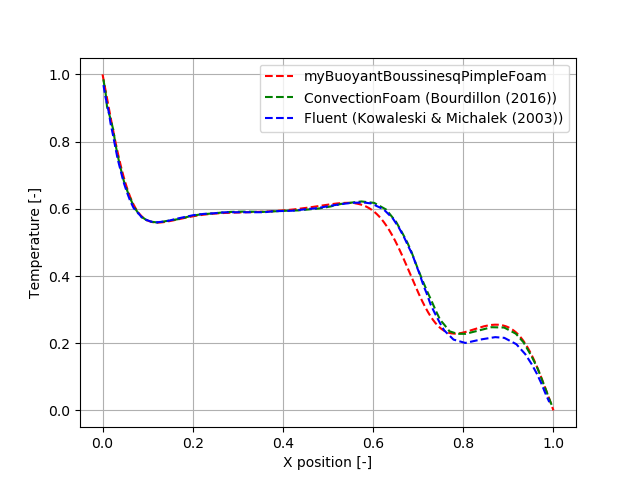
\includegraphics[width=\linewidth]{temperature_xpos_conv.png}\hfill
		\caption{Temperature along horizontal line.} \label{3.4afig}
	\end{subfigure}
	\hfill
	\begin{subfigure}{0.50\textwidth}
		\centering
		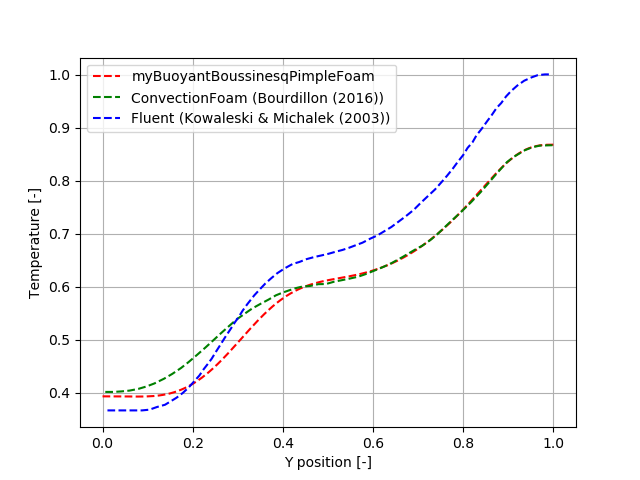
\includegraphics[width=\linewidth]{temperature_ypos_conv.png}	
		\caption{Temperature along vertical line.}\label{3.4bfig}
	\end{subfigure}
	\begin{subfigure}{0.50\textwidth}
		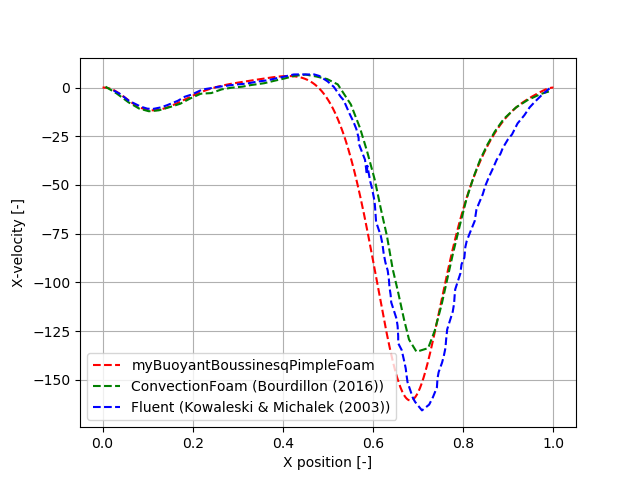
\includegraphics[width=\linewidth]{xvel_xpos_conv.png}\hfill
		\caption{U-velocity along horizontal line.}\label{3.4cfig}
	\end{subfigure}
	\begin{subfigure}{0.50\textwidth}
		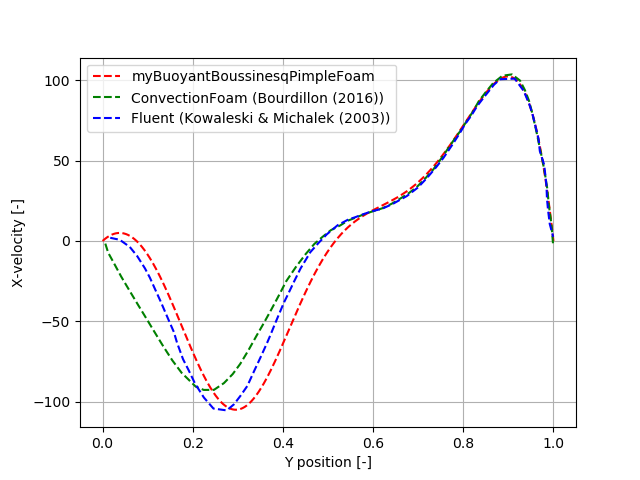
\includegraphics[width=\linewidth]{xvel_ypos_conv.png}	
		\caption{U-velocity along vertical line.}\label{3.4dfig}
	\end{subfigure}
	\begin{subfigure}{0.50\textwidth}
		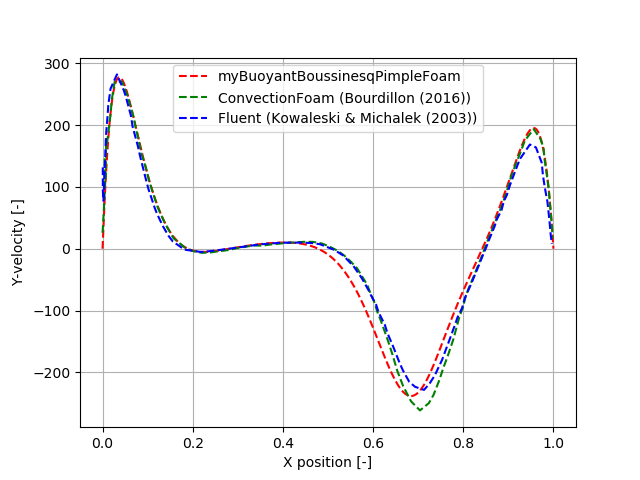
\includegraphics[width=\linewidth]{yvel_xpos_conv.png}\hfill	
		\caption{V-velocity along horizontal line.}\label{3.4efig}
	\end{subfigure}
	\begin{subfigure}{0.50\textwidth}
		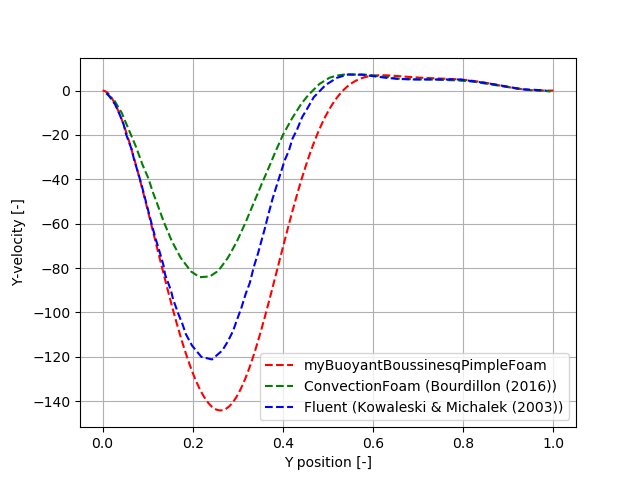
\includegraphics[width=\linewidth]{yvel_ypos_conv.png}	
		\caption{V-velocity along vertical line.}\label{3.4ffig}
	\end{subfigure}
	\caption{Adimensional magnitudes comparison.}
	\label{3.4fig}
\end{figure} 




For the Lee model based on the \textit{Classical Nucleation Theory}, the results are validated against the analytical solution given by the Neumann solutions of the Stefan problem.
\begin{figure}[h!]
	\begin{subfigure}{0.50\textwidth}
		\centering
		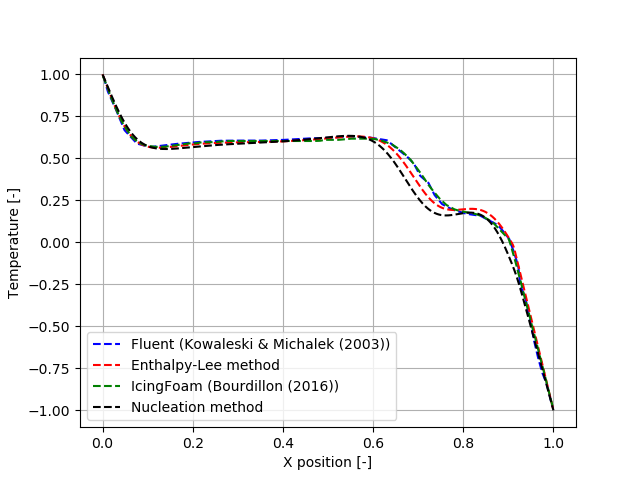
\includegraphics[width=\linewidth]{temperature_xpos_EL.png}\hfill
		\caption{Temperature along horizontal line.} \label{3.5a}
	\end{subfigure}
	\hfill
	\begin{subfigure}{0.50\textwidth}
		\centering
		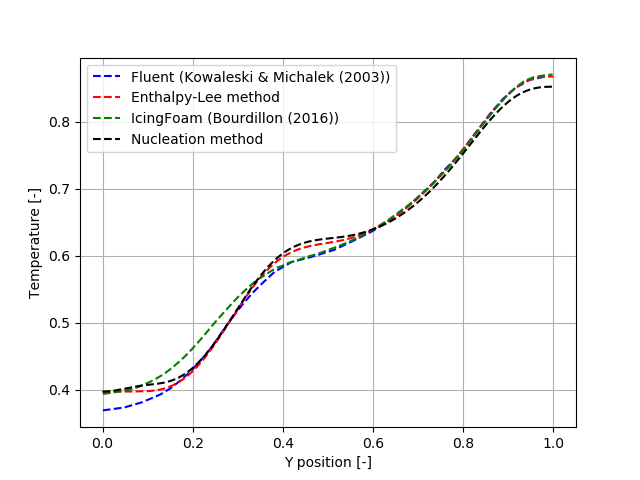
\includegraphics[width=\linewidth]{temperature_ypos_EL.png}	
		\caption{Temperature along vertical line.}\label{3.5b}
	\end{subfigure}
	\begin{subfigure}{0.50\textwidth}
		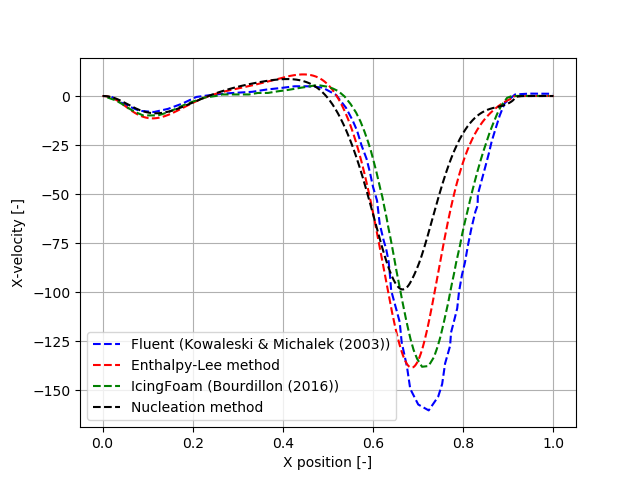
\includegraphics[width=\linewidth]{xvel_xpos_EL.png}\hfill
		\caption{U-velocity along horizontal line.}\label{3.5c}
	\end{subfigure}
	\begin{subfigure}{0.50\textwidth}
		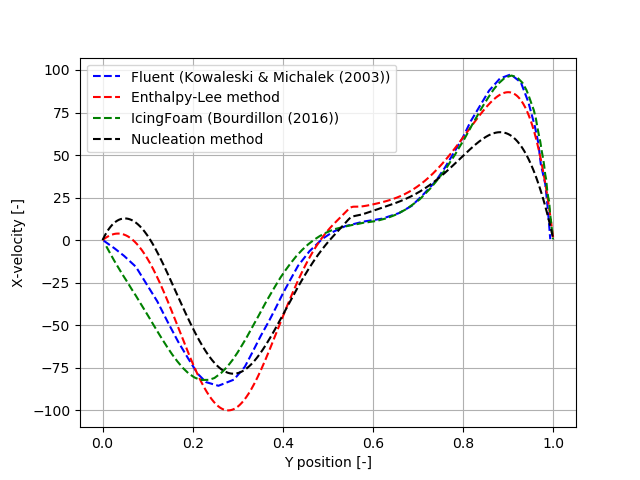
\includegraphics[width=\linewidth]{xvel_ypos_EL.png}	
		\caption{U-velocity along vertical line.}\label{3.5d}
	\end{subfigure}
	\begin{subfigure}{0.50\textwidth}
		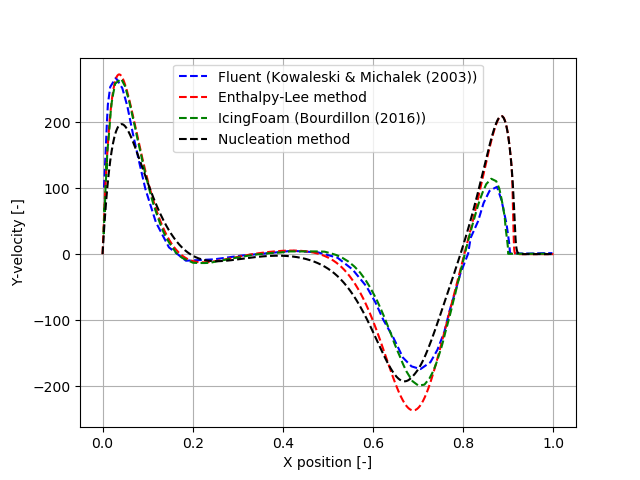
\includegraphics[width=\linewidth]{yvel_xpos_EL.png}\hfill	
		\caption{V-velocity along horizontal line.}\label{3.5e}
	\end{subfigure}
	\begin{subfigure}{0.50\textwidth}
		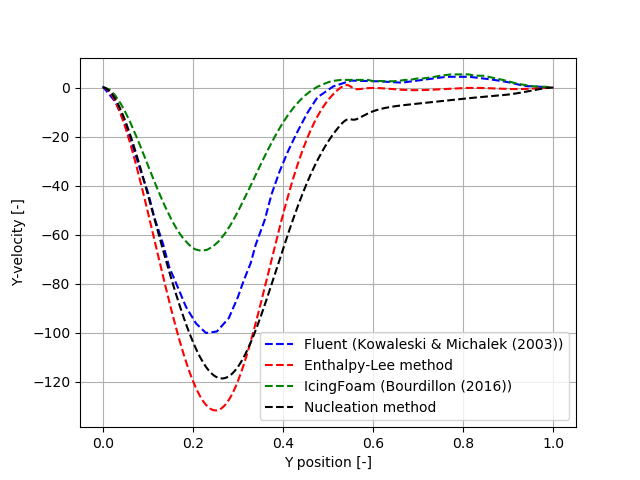
\includegraphics[width=\linewidth]{yvel_ypos_EL.png}	
		\caption{V-velocity along vertical line.}\label{3.5f}
	\end{subfigure}
	\caption{Adimensional magnitudes comparison.}
	\label{3.5}
\end{figure}

\subsubsection{Stefan Problem}
The Stefan problem, is an initial boundary value problem of a parabolic differential equation with discontinuous coefficients on the phase transitions interfaces [\cite{vasilyev_vasilyeva_2020}]. The analytical solution to the classical Stefan problem exists in a limited range of idealized situations. Some of them involve semi-infinite or infinite regions with simple and boundary conditions. Based on the work of \cite{vasilyev_vasilyeva_2020} and \cite{zhao_zhao_xu_2018}, a two-region solidification process in a semi-infinite region is used to study the feasibility of the VOF-Lee model based on the Nucleation Theory.
\subsubsection*{One-dimensional problem}
In seek of simplification, and recalling the 1D problem as shown in the figure:

the initial conditions are expressed as:
\begin{equation}
	u_{0}(x)=u_{0}, \quad t=0, \quad x \in[0, L],
	\label{3.38}
\end{equation}
while the boundary conditions are the shown below:
\begin{equation}
u(0, t)=-15ºC, \quad \frac{\partial u}{\partial x}(L, t)=0, \quad t>0
\label{3.39}
\end{equation}
The discontinuous exact solutions are:
\begin{equation}
	\begin{cases}T_{l}(x, t)=\frac{\operatorname{erfc}\left(\frac{x}{2 \sqrt{a_{1} t}}\right)}{\operatorname{erfc}\left(\lambda \sqrt{\frac{a_{\mathrm{s}}}{a_{1}}}\right)}\left(T_{\mathrm{m}}-T_{0}\right)+T_{0}, & x>\xi(t), \\ 
	T_{\mathrm{s}}(x, t)=\frac{\operatorname{erf}\left(\frac{x}{2 \sqrt{a_{\mathrm{s}} t}}\right)}{\operatorname{erf \cdot\lambda }}\left(T_{\mathrm{m}}-T_{\mathrm{b}}\right)+T_{\mathrm{b}},& x \leq \xi(t)  .\end{cases}
	\label{3.40}
\end{equation}
By using a phase change interface condition, a solution to the trascendental equation may be found:
\begin{equation}
	\frac{e^{-\lambda^{2}}}{\operatorname{erf}(\lambda)}+\frac{k_{\mathrm{l}}}{k_{\mathrm{s}}} \sqrt{\frac{a_{\mathrm{s}}}{a_{1}}} \frac{T_{\mathrm{m}}-T_{0}}{T_{\mathrm{m}}-T_{\mathrm{b}}} \frac{e^{-\frac{a_{\mathrm{s}}}{a_{1}} \lambda^{2}}}{\operatorname{erfc}\left(\lambda \sqrt{\frac{a_{\mathrm{s}}}{a_{1}}}\right)}=\frac{\lambda L \sqrt{\pi}}{c_{\mathrm{ps}}\left(T_{\mathrm{m}}-T_{\mathrm{b}}\right)}
	\label{3.41}
\end{equation}
The secant method is used as the iterative scheme to find the root of the given function with $tol<1e-12$. The root of $\gamma$ is 0.2204835149063661
In the following figures, the accuracy of the method is tested trhough comparison with exact solutions to the Stefan problem.

%The discontinuous exact solution is of the form [\cite{vasilyev_vasilyeva_2020}:
%\begin{equation}
%	u(x, t)= \begin{cases}g\left[\operatorname{erf}\left(\frac{\xi}{2 a_{1} \sqrt{t}}\right)-\operatorname{erf}\left(\frac{x}{2 a_{1} \sqrt{t}}\right)\right] / \operatorname{erf}\left(\frac{\xi}{2 a_{1} \sqrt{t}}\right), & x \geq \xi(t), \\ u_{0}\left[\operatorname{erf}\left(\frac{x}{2 a_{2} \sqrt{t}}\right)-\operatorname{erf}\left(\frac{\xi}{2 a_{2} \sqrt{t}}\right)\right] /\left[1-\operatorname{erf}\left(\frac{\xi}{2 a_{2} \sqrt{t}}\right)\right], & x<\xi(t) .\end{cases}
%\end{equation}
%
%By using a phase change interface condition, it is possible to find a solution to the trascendental equation.
%\begin{equation}
%	\frac{k_{1}}{a_{1}} g \frac{\exp \left(-\left(\frac{\gamma}{2 a_{1}}\right)^{2}\right)}{\operatorname{erf}\left(\frac{\gamma}{2 a_{1}}\right)}+\frac{k_{2}}{a_{2}} u_{0} \frac{\exp \left(-\left(\frac{\gamma}{2 a_{2}}\right)^{2}\right)}{1-\operatorname{erf}\left(\frac{\gamma}{2 a_{2}}\right)}+\gamma D \frac{\sqrt{\pi}}{2}=0
%\end{equation}
%
%The secant method is used as the iterative scheme to find the root of the given function with $tol<1e-12$. The root of $\gamma$ is 0.00032622525325939834
\subsubsection{Interface height}


The evolution of the interface is:
\begin{equation}
X(t)=2 \lambda \sqrt{a_{\mathrm{s}} t}
\label{3.42}
\end{equation}

